\documentclass{ximera}

 

\usepackage{epsfig}

\graphicspath{
  {./}
  {figures/}
}

\usepackage{morewrites}
\makeatletter
\newcommand\subfile[1]{%
\renewcommand{\input}[1]{}%
\begingroup\skip@preamble\otherinput{#1}\endgroup\par\vspace{\topsep}
\let\input\otherinput}
\makeatother

\newcommand{\includeexercises}{\directlua{dofile("/home/jim/linearAlgebra/laode/exercises.lua")}}

%\newcounter{ccounter}
%\setcounter{ccounter}{1}
%\newcommand{\Chapter}[1]{\setcounter{chapter}{\arabic{ccounter}}\chapter{#1}\addtocounter{ccounter}{1}}

%\newcommand{\section}[1]{\section{#1}\setcounter{thm}{0}\setcounter{equation}{0}}

%\renewcommand{\theequation}{\arabic{chapter}.\arabic{section}.\arabic{equation}}
%\renewcommand{\thefigure}{\arabic{chapter}.\arabic{figure}}
%\renewcommand{\thetable}{\arabic{chapter}.\arabic{table}}

%\newcommand{\Sec}[2]{\section{#1}\markright{\arabic{ccounter}.\arabic{section}.#2}\setcounter{equation}{0}\setcounter{thm}{0}\setcounter{figure}{0}}

\newcommand{\Sec}[2]{\section{#1}}

\setcounter{secnumdepth}{2}
%\setcounter{secnumdepth}{1} 

%\newcounter{THM}
%\renewcommand{\theTHM}{\arabic{chapter}.\arabic{section}}

\newcommand{\trademark}{{R\!\!\!\!\!\bigcirc}}
%\newtheorem{exercise}{}

\newcommand{\dfield}{{\sf dfield9}}
\newcommand{\pplane}{{\sf pplane9}}

\newcommand{\EXER}{\section*{Exercises}}%\vspace*{0.2in}\hrule\small\setcounter{exercise}{0}}
\newcommand{\CEXER}{}%\vspace{0.08in}\begin{center}Computer Exercises\end{center}}
\newcommand{\TEXER}{} %\vspace{0.08in}\begin{center}Hand Exercises\end{center}}
\newcommand{\AEXER}{} %\vspace{0.08in}\begin{center}Hand Exercises\end{center}}

% BADBAD: \newcommand{\Bbb}{\bf}

\newcommand{\R}{\mbox{$\Bbb{R}$}}
\newcommand{\C}{\mbox{$\Bbb{C}$}}
\newcommand{\Z}{\mbox{$\Bbb{Z}$}}
\newcommand{\N}{\mbox{$\Bbb{N}$}}
\newcommand{\D}{\mbox{{\bf D}}}
\usepackage{amssymb}
%\newcommand{\qed}{\hfill\mbox{\raggedright$\square$} \vspace{1ex}}
%\newcommand{\proof}{\noindent {\bf Proof:} \hspace{0.1in}}

\newcommand{\setmin}{\;\mbox{--}\;}
\newcommand{\Matlab}{{M\small{AT\-LAB}} }
\newcommand{\Matlabp}{{M\small{AT\-LAB}}}
\newcommand{\computer}{\Matlab Instructions}
\newcommand{\half}{\mbox{$\frac{1}{2}$}}
\newcommand{\compose}{\raisebox{.15ex}{\mbox{{\scriptsize$\circ$}}}}
\newcommand{\AND}{\quad\mbox{and}\quad}
\newcommand{\vect}[2]{\left(\begin{array}{c} #1_1 \\ \vdots \\
 #1_{#2}\end{array}\right)}
\newcommand{\mattwo}[4]{\left(\begin{array}{rr} #1 & #2\\ #3
&#4\end{array}\right)}
\newcommand{\mattwoc}[4]{\left(\begin{array}{cc} #1 & #2\\ #3
&#4\end{array}\right)}
\newcommand{\vectwo}[2]{\left(\begin{array}{r} #1 \\ #2\end{array}\right)}
\newcommand{\vectwoc}[2]{\left(\begin{array}{c} #1 \\ #2\end{array}\right)}

\newcommand{\ignore}[1]{}


\newcommand{\inv}{^{-1}}
\newcommand{\CC}{{\cal C}}
\newcommand{\CCone}{\CC^1}
\newcommand{\Span}{{\rm span}}
\newcommand{\rank}{{\rm rank}}
\newcommand{\trace}{{\rm tr}}
\newcommand{\RE}{{\rm Re}}
\newcommand{\IM}{{\rm Im}}
\newcommand{\nulls}{{\rm null\;space}}

\newcommand{\dps}{\displaystyle}
\newcommand{\arraystart}{\renewcommand{\arraystretch}{1.8}}
\newcommand{\arrayfinish}{\renewcommand{\arraystretch}{1.2}}
\newcommand{\Start}[1]{\vspace{0.08in}\noindent {\bf Section~\ref{#1}}}
\newcommand{\exer}[1]{\noindent {\bf \ref{#1}}}
\newcommand{\ans}{}
\newcommand{\matthree}[9]{\left(\begin{array}{rrr} #1 & #2 & #3 \\ #4 & #5 & #6
\\ #7 & #8 & #9\end{array}\right)}
\newcommand{\cvectwo}[2]{\left(\begin{array}{c} #1 \\ #2\end{array}\right)}
\newcommand{\cmatthree}[9]{\left(\begin{array}{ccc} #1 & #2 & #3 \\ #4 & #5 &
#6 \\ #7 & #8 & #9\end{array}\right)}
\newcommand{\vecthree}[3]{\left(\begin{array}{r} #1 \\ #2 \\
#3\end{array}\right)}
\newcommand{\cvecthree}[3]{\left(\begin{array}{c} #1 \\ #2 \\
#3\end{array}\right)}
\newcommand{\cmattwo}[4]{\left(\begin{array}{cc} #1 & #2\\ #3
&#4\end{array}\right)}

\newcommand{\Matrix}[1]{\ensuremath{\left(\begin{array}{rrrrrrrrrrrrrrrrrr} #1 \end{array}\right)}}

\newcommand{\Matrixc}[1]{\ensuremath{\left(\begin{array}{cccccccccccc} #1 \end{array}\right)}}



\renewcommand{\labelenumi}{\theenumi)}
\newenvironment{enumeratea}%
{\begingroup
 \renewcommand{\theenumi}{\alph{enumi}}
 \renewcommand{\labelenumi}{(\theenumi)}
 \begin{enumerate}}
 {\end{enumerate}\endgroup}



\newcounter{help}
\renewcommand{\thehelp}{\thesection.\arabic{equation}}

%\newenvironment{equation*}%
%{\renewcommand\endequation{\eqno (\theequation)* $$}%
%   \begin{equation}}%
%   {\end{equation}\renewcommand\endequation{\eqno \@eqnnum
%$$\global\@ignoretrue}}

%\input{psfig.tex}

\author{Martin Golubitsky and Michael Dellnitz}

%\newenvironment{matlabEquation}%
%{\renewcommand\endequation{\eqno (\theequation*) $$}%
%   \begin{equation}}%
%   {\end{equation}\renewcommand\endequation{\eqno \@eqnnum
% $$\global\@ignoretrue}}

\newcommand{\soln}{\textbf{Solution:} }
\newcommand{\exercap}[1]{\centerline{Figure~\ref{#1}}}
\newcommand{\exercaptwo}[1]{\centerline{Figure~\ref{#1}a\hspace{2.1in}
Figure~\ref{#1}b}}
\newcommand{\exercapthree}[1]{\centerline{Figure~\ref{#1}a\hspace{1.2in}
Figure~\ref{#1}b\hspace{1.2in}Figure~\ref{#1}c}}
\newcommand{\para}{\hspace{0.4in}}

\renewenvironment{solution}{\suppress}{\endsuppress}

\ifxake
\newenvironment{matlabEquation}{\begin{equation}}{\end{equation}}
\else
\newenvironment{matlabEquation}%
{\let\oldtheequation\theequation\renewcommand{\theequation}{\oldtheequation*}\begin{equation}}%
  {\end{equation}\let\theequation\oldtheequation}
\fi

\makeatother


\title{Stylized Phase Portraits}

\begin{document}
\begin{abstract}
\end{abstract}
\maketitle

  \label{S:SPP}
\index{stylized phase portrait}\index{phase!portrait!stylized}


In Section~\ref{S:linearization} we discussed phase portraits of systems with 
equilibria but without periodic solutions.  In Section~\ref{S:periodic} we 
discussed briefly certain planar systems having limit cycles.  In this 
section we combine the discussions on equilibria and periodic solutions; 
together these discussions allow us to give a strategy for determining 
numerically the phase portraits of a broad class of planar autonomous 
differential equations --- the Morse-Smale differential equations.
 
Planar phase portraits indicate all equilibria, periodic
solutions, and connecting trajectories.  The simplest phase
portraits are those that describe the dynamics of differential
equations satisfying the following assumptions: \index{hyperbolic}
\begin{itemize}
\item	All equilibria are hyperbolic.
\item	All periodic solutions are limit cycles.
\item	There are no trajectories connecting two saddle points.
\end{itemize}
A planar system of differential equations that satisfies these
three conditions is called a {\em Morse-Smale\/} system.  
\index{Morse-Smale system}

\begin{definition} \label{D:stylized}
A {\em stylized phase portrait\/} of a planar autonomous system
of differential equations is a picture illustrating all
equilibria and their type, all limit cycles, and all connecting
trajectories.
\end{definition}\index{stylized phase portrait}\index{phase!portrait!stylized}

Generally, it is not an easy task to draw the stylized phase
portrait of a differential equation.  However, using {\sf pplane8\/} 
we can attempt to draw the phase portrait of a
Morse-Smale system on a given rectangle in the following way.
\begin{enumerate}
\item Using both analysis and numerics, find the equilibria of
the differential equation.
\item Mark these equilibria and their type.  
\item Draw the stable and unstable orbits of saddles.  
\index{saddle!stable and unstable orbits}
\item Determine the number and stability of limit cycles.  
\end{enumerate}
Putting this information together allows us to draw planar phase
portraits.

\subsection*{The {\pplane} Default Equation}

As an example, we discuss the stylized phase portrait of the 
{\pplane}\index{\computer!pplane8} default equation:
\begin{equation}  \label{e:default}
\begin{array}{rcl}
\dot{x} & = & 2x-y+3(x^2-y^2)+2xy \\
\dot{y} & = & x-3y-3(x^2-y^2)+3xy
\end{array}
\end{equation} 
Our goal is to draw the stylized phase portrait of this system
of differential equations on some rectangle in the plane, and we
choose the default rectangle: $-2\leq x\leq 4$, $-4\leq y\leq 2$.

Inspection of \eqref{e:default} shows that the origin\index{origin} 
is an equilibrium.  By clicking on the {\sf Find an equilibrium point}
button, we see that the origin is a saddle.  By clicking on the
{\sf plot stable and unstable orbits} button and then clicking
on the mouse when the cross hairs are near the origin, {\sf
pplane8} plots the stable and unstable orbits of this saddle.
See Figure~\ref{F:default0}.

\begin{figure*}[htb]
           \centerline{%
	   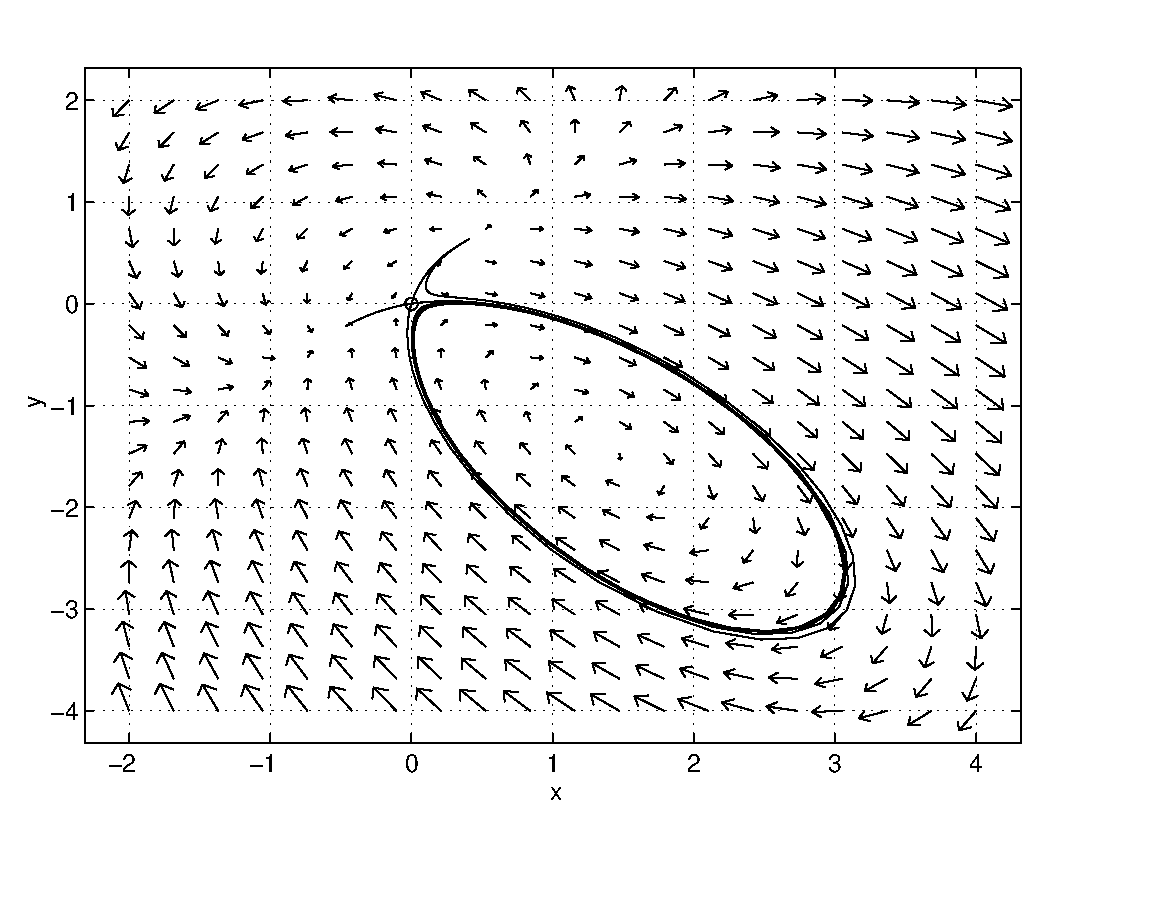
\psfig{file=../figures/default0.eps,width=3.2in}
	   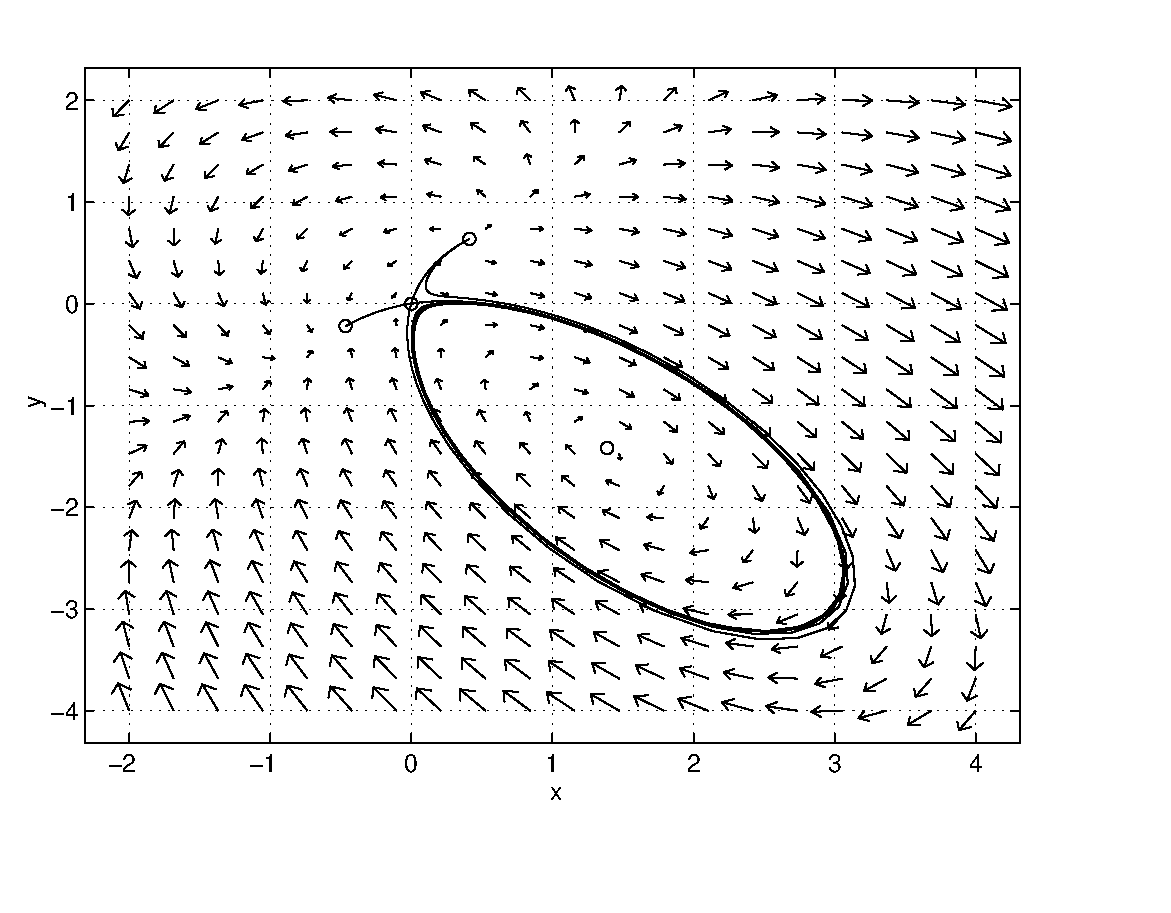
\psfig{file=../figures/default1.eps,width=3.2in}}
           \caption{(Left) Stable and unstable orbits of the saddle at
		the origin in \protect\eqref{e:default}. (Right) Picture 
		of \protect\eqref{e:default} with equilibria added.}
           \label{F:default0}
\end{figure*}
 
This calculation reveals several interesting features in the
phase portrait of \eqref{e:default}.  First, both stable orbits limit on the 
same equilibrium, and that equilibrium is near $(0.5,0.5)$.  Second, one 
unstable orbit limits on an equilibrium near $(-0.5,-0.2)$, while the other 
unstable orbit limits on what appears to be a limit cycle.  It follows from 
Theorem~\ref{T:PB} that there must be an equilibrium inside this limit cycle 
--- probably near $(1.3,-1.3)$.  Using the information and the {\sf
Find an equilibrium point} button, we can locate three
equilibria:
\begin{itemize}
\item	A nodal sink at $(-0.4661,-0.2209)$,
\item	A nodal source at $(0.4125,0.6386)$,
\item	A spiral source at $(1.387,-1.418)$. 
\end{itemize}
Entering these equilibria yields the phase portrait in 
Figure~\ref{F:default0} (right). 

We now draw the stylized phase portrait\index{stylized phase portrait}
\index{phase!portrait!stylized} for \eqref{e:default},
indicating the four equilibria and their type, the periodic
solutions, and the connecting trajectories. See
Figure~\ref{F:default2} (right).  A picture with additional 
trajectories is shown on the left of that figure.

\begin{figure*}[htb]
           \centerline{%
	   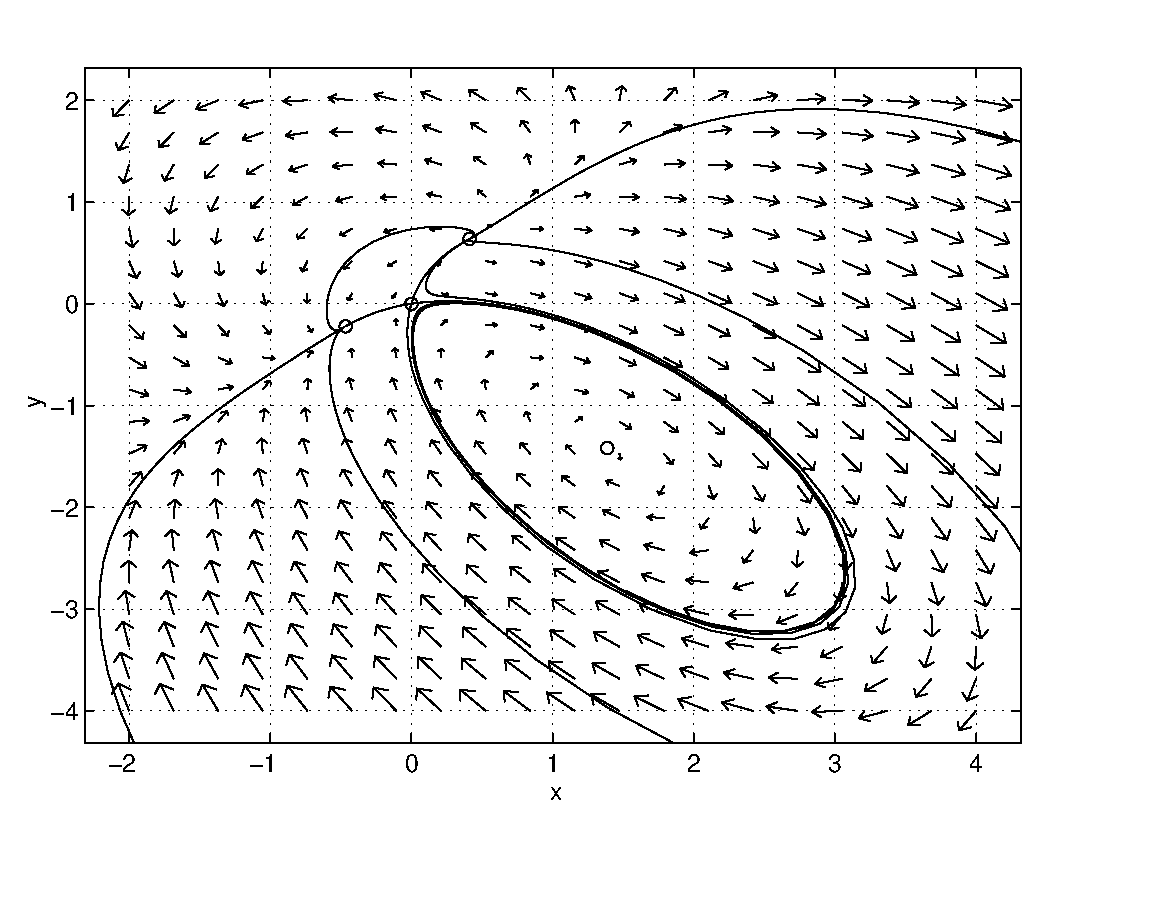
\psfig{file=../figures/default2.eps,width=3.0in}
	   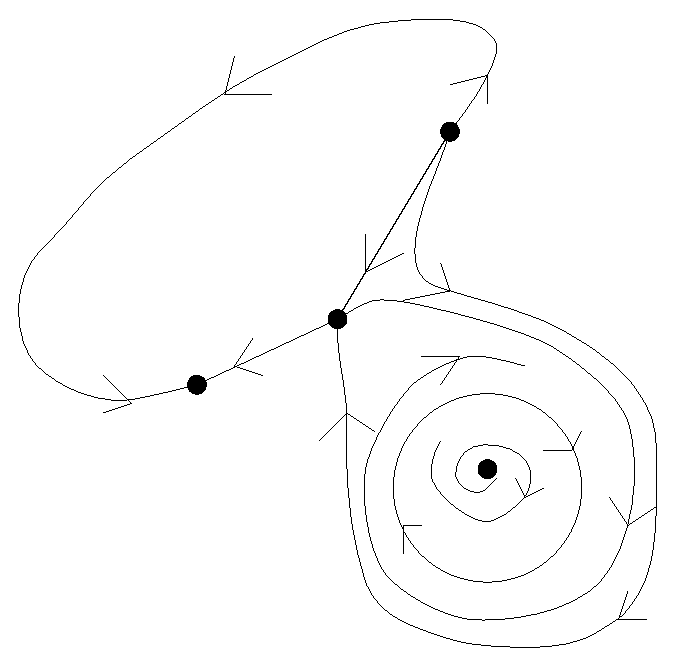
\psfig{file=../figures/default4.eps,height=2.2in}
		}
           \caption{(Left) Additional trajectories of 
\protect\eqref{e:default}. (Right) Stylized phase portrait
indicating equilibria, periodic solutions and connecting trajectories.}
           \label{F:default2}
\end{figure*}

It is reasonable to wonder whether this somewhat ad hoc process
for finding the stylized phase portrait will always work.  The
simple answer is {\em no} --- but much progress can be made if
one proceeds cautiously.  

For example, one numerical difficulty appears in the analysis of
the default system \eqref{e:default}.  Clicking inside the limit
cycle, shows a trajectory that spirals to a limit cycle in
forward time, as expected. In backward time, however, the
trajectory spirals towards the spiral source --- but never makes
it --- and {\pplane} indicates the possible existence of a
second periodic solution.  In fact, no such periodic solution
exists. This point can be clarified using the zoom feature near
the spiral source.  These numerical calculations verify that the 
default system \eqref{e:default} is Morse-Smale.

\EXER

\includeexercises

\end{document}
